
\subsection{Ejercicio 10}

Dadas las implementaciones de $ShedLottery$, con o sin tickets compensatorios (respectivamente en $sched\_lottery.cpp$ y $sched\_lottery\_base.cpp$), el ejercicio nos propone ponerlas a prueba y compararlas, relacion\'andolas con la problem\'atica que presentaban los autores y verificar si los tickets compensatorios son una soluci\'on viable. 

\vspace{2mm}

Para esto generamos dos lotes distintos: \textbf{Lote7}, que consta de 3 tareas intensivas de CPU y una tarea de I/O bloqueante, y para comprobar que el mecanismo funciona con varias tareas bloqueadas al mismo tiempo, el lote \textbf{Lote8} con 2 tareas intenstivas de CPU y 2 bloqueantes.

\vspace{2mm}
\textbf{Lote7:}

\begin{lstlisting}[numbers=none]
@0:
*3 TaskCPU 50
*1 TaskConsola 50 1 2
\end{lstlisting}

\vspace{2mm}
\textbf{Lote8:}

\begin{lstlisting}[numbers=none]
@0:
*2 TaskCPU 50
*2 TaskConsola 25 1 2
\end{lstlisting}

\subsubsection{Experimentos: Lote 7}

\vspace{2mm}

Los experimentos fueron realizados con los par\'ametros: \textbf{semilla} aleatoria(pero la misma para cada comparaci\'on entre schedulers), \textbf{quantum} de tres ticks, \textbf{bloqueos} de un tick (con el objetivo de generar muchos cambios de contexto y tener m\'as casos de an\'alisis), \textbf{cantidad de procesadores} de uno y costo de \textbf{cambio de contexto} de cero, para hacer m\'as sencillo el an\'alisis y no agregar variables que no aportan al experimento.

\vspace{2mm}

\textbf{Caso1:}

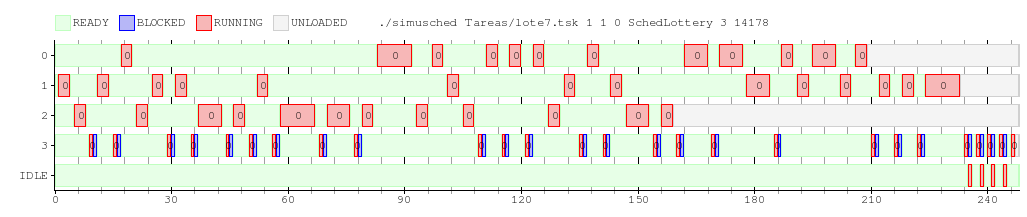
\includegraphics[width=1\textwidth]{./Graficos/Ej10v2/Task7/ej9_1.png}
\begin{center}
 \textit{Scheduler = Compensatorio, Semilla = 14178}.
\end{center}


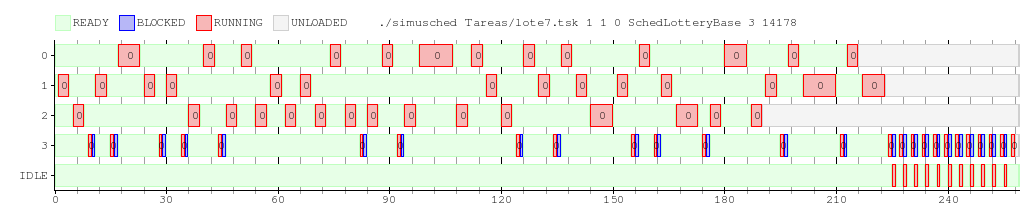
\includegraphics[width=1\textwidth]{./Graficos/Ej10v2/Task7/ej9_1_base.png}
\begin{center}
 \textit{Scheduler = No Compensatorio, Semilla = 14178}.
\end{center}

\vspace{2mm}


Pueden notarse las 3 tareas intensivas de CPU y la tarea I/O, que procesa 1 tick y se bloquea. Aqui vemos como, en el caso sin compensation tickets, la tarea se bloquea, perdiendo $2/3$ de su quantum y luego vuelve a obtener el cpu muchos ticks despues, perdiendo tiempo de procesamiento. Esto se nota claramente al ver que m\'as de la mitad de su tiempo de procesamiento se produce al final de la simulaci\'on.

\vspace{2mm}

En el caso con compensation tickets, puede notarse como luego de bloquearse, en el siguiente cambio de contexto a su desbloqueo vuelve a obtener la cpu en varios casos, producto de su aumento de probabilidad gracias a los compensation tickets. Pueden compararse adem\'as ambos finales de las simulaciones y notar que, en la simulaci\'on con tickets compensatorios, restan muchos menos ticks de la tarea I/O por procesar.

\vspace{2mm}
\textbf{Caso2:}

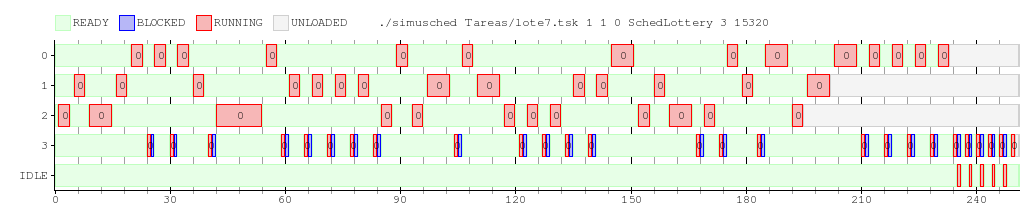
\includegraphics[width=1\textwidth]{./Graficos/Ej10v2/Task7/ej9_2.png}
\begin{center}
 \textit{Scheduler = Compensatorio, Semilla = 15320}.
\end{center}


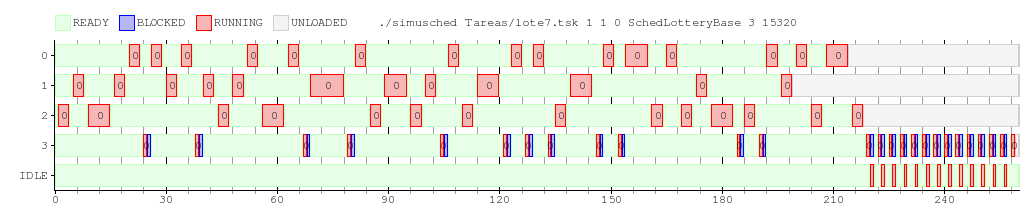
\includegraphics[width=1\textwidth]{./Graficos/Ej10v2/Task7/ej9_2_base.png}
\begin{center}
 \textit{Scheduler = No Compensatorio, Semilla = 15320}.
\end{center}

En este caso pueden observarse tambi\'en bursts de la tarea I/O, y puede notarse adem\'as que una vez que la tarea pierde la asignaci\'on de la CPU en su tick compensado, es poco probable que la vuelva a obtener por un per\'iodo, ya que debido a la implementaci\'on de tickets compensatorios, si una tarea compensada pierde la asignac\'on, sus tickets compensatorios son retirados de todas formas.

\vspace{2mm}
\textbf{Caso3:}


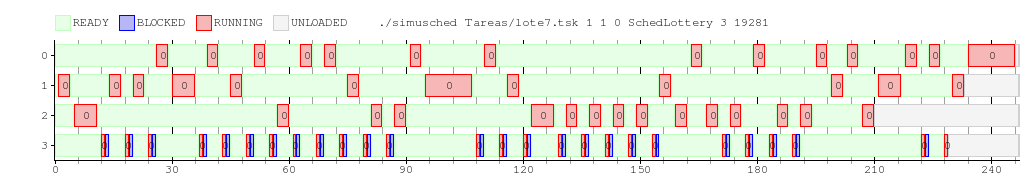
\includegraphics[width=1\textwidth]{./Graficos/Ej10v2/Task7/ej9_3.png}
\begin{center}
 \textit{Scheduler = Compensatorio, Semilla = 19281}.
\end{center}


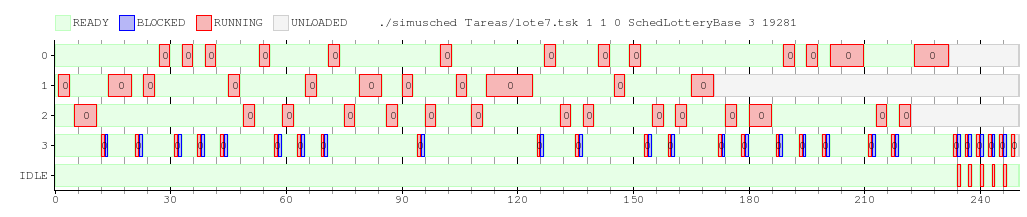
\includegraphics[width=1\textwidth]{./Graficos/Ej10v2/Task7/ej9_3_base.png}
\begin{center}
 \textit{Scheduler = No Compensatorio, Semilla = 19281}.
\end{center}

En este caso se aprecia claramente que la implementaci\'on de tickets compensatorios equilibra efectivamente la asignaci\'on de CPU, ya que comparado con la simulaci\'on no compensada, donde la tarea I/O debe terminar su ejecuci\'on al \'ultimo, en el caso compensado esta tarea recibe la asignaci\'on del CPU mucho m\'as frecuentemente, e incluso finaliza su ejecuci\'on \textbf{antes} que dos de las dem\'as.

\vspace{2mm}
\textbf{Caso4:}


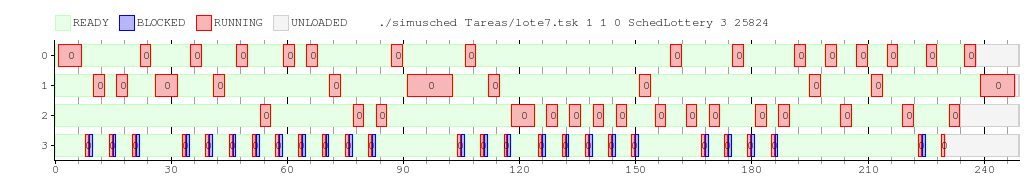
\includegraphics[width=1\textwidth]{./Graficos/Ej10v2/Task7/ej9_4.png}
\begin{center}
 \textit{Scheduler = Compensatorio, Semilla = 25824}.
\end{center}


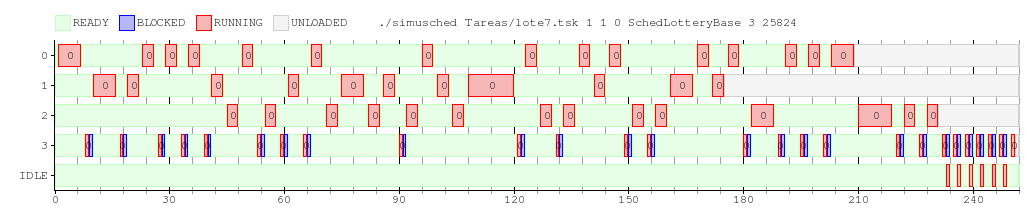
\includegraphics[width=1\textwidth]{./Graficos/Ej10v2/Task7/ej9_4_base.png}
\begin{center}
 \textit{Scheduler = No Compensatorio, Semilla = 25824}.
\end{center}

El \'ultimo caso analizado refleja correctamente todo lo anteriormente planteado. De esta forma concluimos en que en el caso de una tarea que se bloquea frecuentemente y compite por el CPU contra varias otras de uso intensivo de \'este, la implementaci\'on de tickets compensatorios logra homogeneizar la asignaci\'on y aprovechar ciclos de procesamiento.

\subsubsection{Experimentos: Lote 8}

\vspace{2mm}

\textbf{Caso1:}

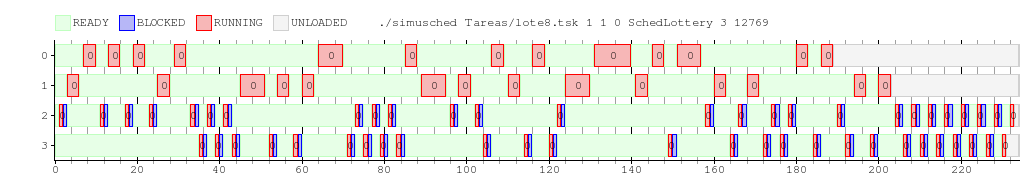
\includegraphics[width=1\textwidth]{./Graficos/Ej10v2/Task8/ej9_1.png}
\begin{center}
 \textit{Scheduler = Compensatorio, Semilla = 14178}.
\end{center}


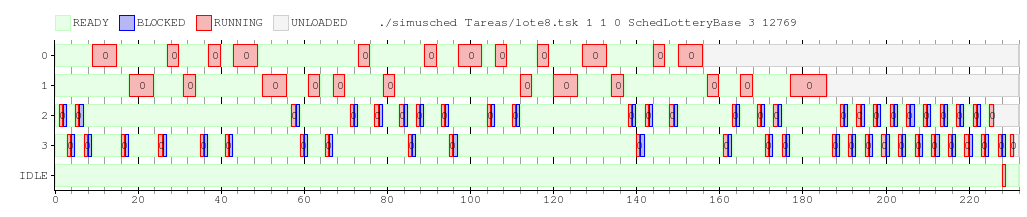
\includegraphics[width=1\textwidth]{./Graficos/Ej10v2/Task8/ej9_1_base.png}
\begin{center}
 \textit{Scheduler = No Compensatorio, Semilla = 14178}.
\end{center}